\documentclass[11pt, table]{beamer}
%\usepackage[table,x11names]{xcolor}
%\usepackage[utf8]{inputenc}
%\usepackage[T1]{fontenc}
%\usepackage{multirow}
%\usepackage{calc}
%\usepackage{array}
\usepackage{graphicx}
%\usepackage{multirow}

\newcommand{\p}{\pause}


\usetheme{default}

\newcommand\MyBox[2]{
	\fbox{\lower0.75cm
		\vbox to 1.7cm{\vfil
			\hbox to 1.7cm{\hfil\parbox{1.4cm}{#1\\#2}\hfil}
			\vfil}%
	}%
}

\begin{document}
	\title{Estimation, Part 1:\newline Sampling Distributions}
	\date{}
	\begin{frame}[plain]
	\maketitle
\end{frame}

\begin{frame}
\frametitle{Estimation}

When doing statistics, the goal is usually to \emph{infer} something about a population \emph{parameter} using only a sample from that population.
\vspace{0.25in}\p

\textbf{Examples:}
\begin{itemize}
	\item Estimating the average household income in Davidson County, based on a sample.\p
	\item Predict who will win an upcoming election, based on a poll.
\end{itemize}
\end{frame}

\begin{frame}[t]
\frametitle{Estimation}
	We are trying to say something about the entire population just be examining a subset.
\vspace{0.25in}

	\begin{center}
	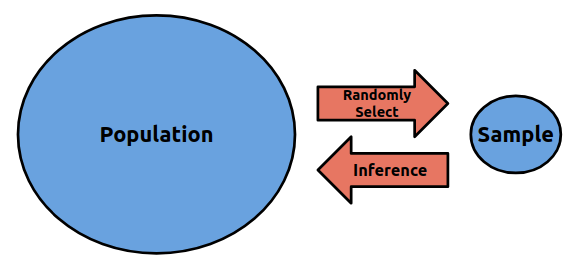
\includegraphics[width = 0.9\textwidth]{images/pop_sample.png}
	\end{center}
\end{frame}

\begin{frame}
\frametitle{Estimation}
One option that we have to to report a \textbf{point estimate}. That is, we can report just a single number as our estimate for the population parameter.

\vspace{0.25in}
For example, we might survey 100 households in Davidson County and estimate, based on our sample, that the average household income in Davidson County is \$43,000.
\end{frame}

\begin{frame}
\frametitle{Estimation}
However, if we are only reporting a single number, we are very unlikely to be correct. We would usually be better off reporting our estimate, along with how close it is likely to be to the correct number.\p

\vspace{\stretch{1}}
To improve our income estimate above, we might say that we are fairly confident that our original estimate of household income being \$43,000 is off by no more that \$1,500. If we do this, we are indicating that our estimate has \textbf{margin of error} \$1,500.\p

\vspace{\stretch{1}}
We can frame our estimate and margin of error in another way, by saying that we are confident that the true mean household income is in the interval
$$\$43,000 \pm \$1,500$$\p

\vspace{\stretch{1}}
That is, we are highly confident that the true population mean is between \$41,500 and \$44,500.

\end{frame}

\begin{frame}
\frametitle{Estimation}

Another way to write this is that a confidence interval for $\mu$ is given by

$$41500 < \mu < 44500$$

Here, $\mu$ represents the true average household income of Davidson County.
\end{frame}

\begin{frame}
\frametitle{Confidence Intervals}
A \textbf{confidence interval} is an interval that is used to estimate the value of a parameter.\p

\vspace{0.25in}
Associated with a confidence interval is a \textbf{confidence level}.
A confidence level is a percentage between 0\% and 100\% that measures the success rate of the method used to construct the confidence interval. If we were to draw many samples and use each one to construct a confidence interval, then in the long run, the percentage of confidence intervals that cover the true value would be equal to the confidence level.\p

\vspace{0.25in}
To make our household income estimate into a true confidence interval, we need to attach a confidence level. For example, I could say that I am 95\% confident that the true mean household income is in the interval \$43,000 $\pm$ \$1,500.
\end{frame}

\begin{frame}
\frametitle{Confidence Intervals}
The general formula for a confidence interval is
$$\text{point estimate} \pm \text{margin of error}$$
\vspace{0.25in}\p

For example, for the Davidson County mean household income, our point estimate was \$43,000 and our margin of error was \$1,500.
\end{frame}

\begin{frame}
\frametitle{Confidence Intervals}
How do we find the margin of error?
\vspace{0.2in}

To come up with a general recipe, we have to temporarily pretend like we know something about the entire population of interest.
\vspace{0.2in}

Let's pretend that in Davidson County, household incomes are distributed normally with a mean of \$44,100 and a standard deviation of \$12,890. (Note: this is not a good approximation of income distribution, but this is only a thought experiment.)

\begin{center}
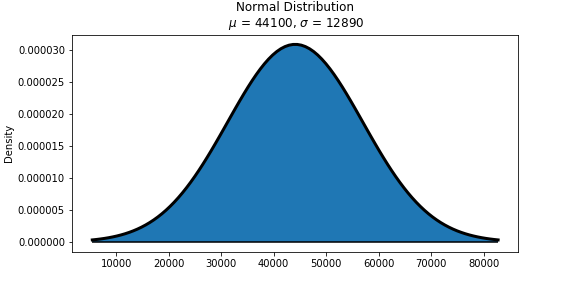
\includegraphics[width = 3in]{images/income_plot.png}
\end{center}
\end{frame}

\begin{frame}
\frametitle{Confidence Intervals}

Note that the pdf describes the probability of a \emph{single (random) observation} landing in a particular range.

Let's take a random sample of size 10 and see where it lands on this distribution.
\begin{center}
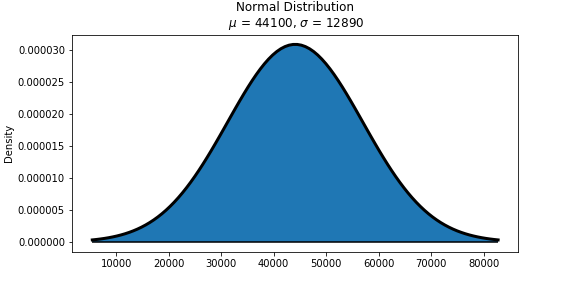
\includegraphics[width = 3in]{images/income_plot.png}
\end{center}

\end{frame}

\begin{frame}
\frametitle{Confidence Intervals}
Let's take a random sample of size 10 and see where it lands on this distribution.
\begin{center}
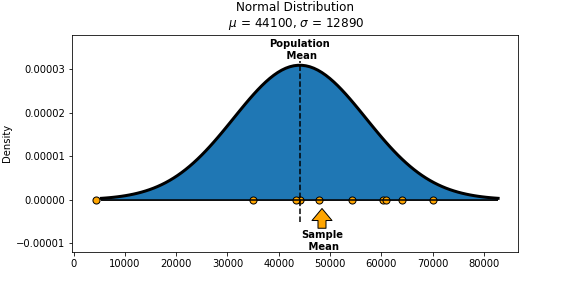
\includegraphics[width = 3in]{images/sample_plot_1.png}
\end{center}
Even though individual elements of the sample can be quite far from the population mean, the sample mean ends up close to (but not exactly equal to) the population mean.

Let's see what happens if we take a different sample of size 10.
\end{frame}

\begin{frame}
\frametitle{Confidence Intervals}
Let's take a random sample of size 10 and see where it lands on this distribution.
\begin{center}
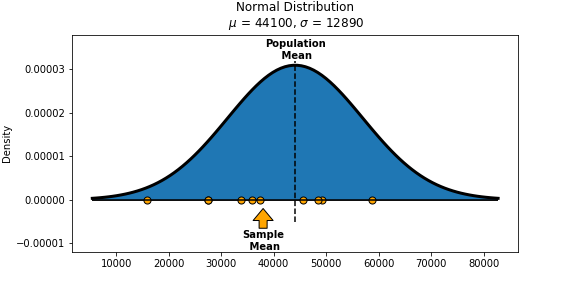
\includegraphics[width = 3in]{images/sample_plot_2.png}
\end{center}
This time the sample mean ends up further away from the population mean.

Let's see what happens if we take a different sample of size 10.
\end{frame}

\begin{frame}
\frametitle{Confidence Intervals}
Let's take a random sample of size 10 and see where it lands on this distribution.
\begin{center}
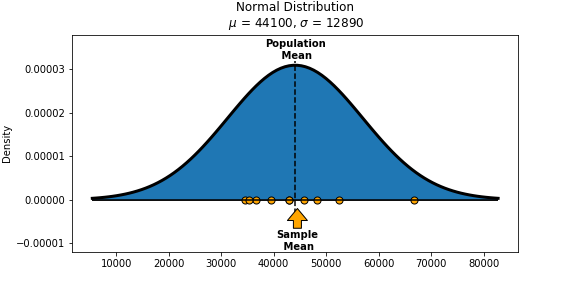
\includegraphics[width = 3in]{images/sample_plot_3.png}
\end{center}
This time we end up quite close (but not exactly equal to) the population mean.

Let's see what happens if we take a different sample of size 10.
\end{frame}

\begin{frame}
\frametitle{Confidence Intervals}
Let's take a random sample of size 10 and see where it lands on this distribution.
\begin{center}
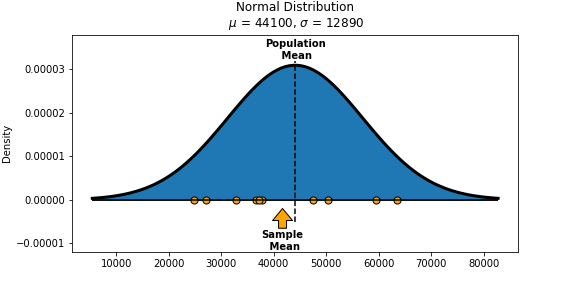
\includegraphics[width = 3in]{images/sample_plot_4.png}
\end{center}
Again, we end up close to the population mean.
\end{frame}

\begin{frame}
\frametitle{Confidence Intervals}
In practice, the difficult thing is that we don't get to know the true population distribution, so we can't see how close our sample is. We really only get a single shot and have to try and determine how close we are likely to be.
\vspace{0.2in}

From what we've seen, the sample means have been pretty good estimates of the population mean, but there is some variance.
\vspace{0.2in}

We can treat the sample mean $\bar{x}$ as a random variable and try to understand the distribution of $\bar{x}$.

\end{frame}

\begin{frame}
\frametitle{Confidence Intervals}
Let's try and see what this distribution looks like. In the following picture, each red dot corresponds to the sample mean from a sample of size 10. There were 500 different samples picked.

\begin{center}
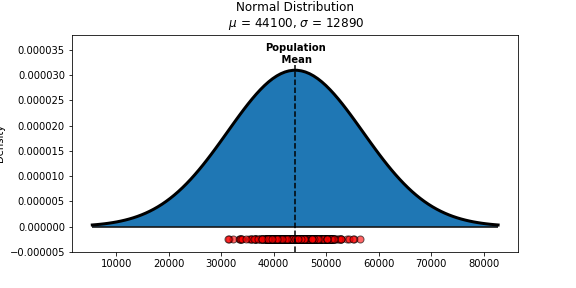
\includegraphics[width = 3in]{images/sampling_distribution.png}
\end{center}

Notice that not a single time out of 500 samples was the sample mean less than 30000 or above 60000.
\end{frame}

\begin{frame}
\frametitle{Confidence Intervals}
Let's look at a KDE of the distribution of sample means.

\begin{center}
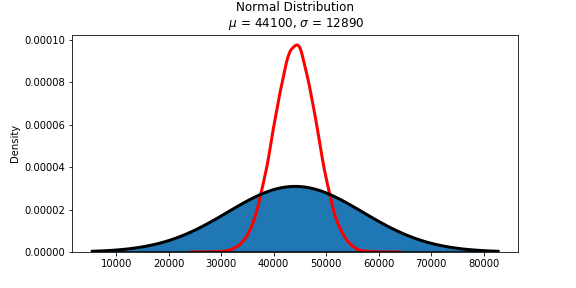
\includegraphics[width = 3in]{images/sd_kde.png}
\end{center}

What we can see is that the distribution of sample means is centered around the population mean but is much narrower than the population distribution.
\end{frame}

\begin{frame}
\frametitle{Confidence Intervals}
Remember that the distribution we were looking at was for samples of size 10. What if we increase the sample size to 100?

\begin{center}
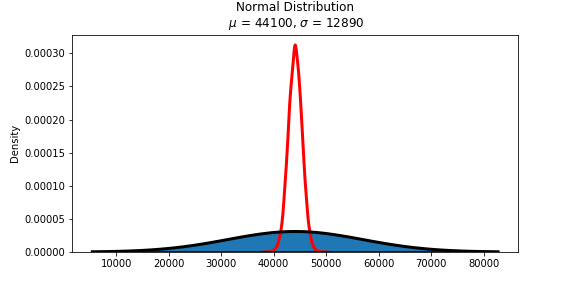
\includegraphics[width = 3in]{images/sd_kde_larger.png}
\end{center}

We get an even narrower distribution around the mean.
\end{frame}

\begin{frame}
\frametitle{Confidence Intervals}
What if we increase the sample size to 500?

\begin{center}
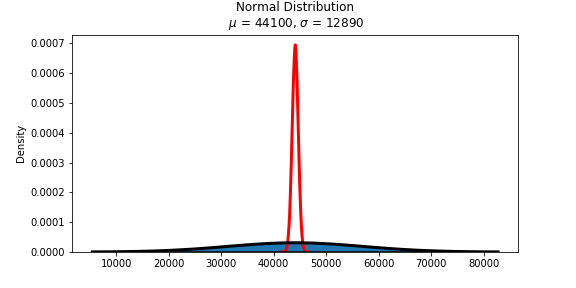
\includegraphics[width = 3in]{images/sd_kde_even_larger.png}
\end{center}

We can see that at this sample size, there is not a lot of variance at all in the sampling distribution. 
\vspace{0.1in}

This can give us a pretty good idea of how far off our estimate is likely to be if we use the sample mean. (Insert widget demo here)
\end{frame}

\begin{frame}
\frametitle{Confidence Intervals}
So the widget shows us that if we know what the sampling distribution of the mean (or whatever parameter we are interested in) looks like, we can use this to construct our confidence interval. \p
\vspace{0.2in}

\textbf{Central Limit Theorem:} For the random variable $\bar{x}$, the sample mean of a random sample of size $n$ from a given population having mean $\mu$ and standard deviation $\sigma$, if $n$ is sufficiently large, then the distribution of $\bar{x}$ is approximately normal with mean $\mu$ and standard deviation $\frac{\sigma}{\sqrt{n}}$.
\vspace{0.2in}

Thus, $\frac{\bar{x} - \mu}{\sigma / \sqrt{n}}$ approximately follows a standard normal distribution.
\end{frame}

\begin{frame}
\frametitle{Confidence Intervals}
There is a problem with using the Central Limit Theorem. In order to use it to construct a confidence interval, we need to know $\frac{\sigma}{\sqrt{n}}$. But if we don't know the population mean $\mu$, why would we know the population standard deviation $\sigma$. The best we could do would be to approximate it with the sample standard deviation, $s$. 
\vspace{0.2in}

\textbf{Fact:} If either the population is normally distributed or we have a large enough sample (usually 30 will do), then 
$$\frac{\bar{x} - \mu}{s / \sqrt{n}}$$
follows a Student's $t$-distribution with $n-1$ degrees of freedom.
\end{frame}

\begin{frame}
\frametitle{Confidence Intervals}
The family of Student's $t$-distribution is a family of symmetric, bell-shaped distributions, which are similar to normal distributions, but have wider tails. That is, more extreme observations are more common.
\vspace{0.2in}
\end{frame}

\begin{frame}
\frametitle{Confidence Interval}
\textbf{Big Idea:} If we want a 95\% confidence interval, we just need to find the distance $t_{0.025}$ from the center of the $t$ distribution with $n-1$ degrees of freedom to the point where the area to the right is $0.025$ (that is, $t_{0.025}$ is the 97.5th percentile).
\vspace{0.1in}

Once we know $t_{0.25}$, we can get the margin of error by multiplying by the standard deviation of the sampling distribution, $\frac{\sigma}{\sqrt{n}}$. This means that our confidence interval is
$$\bar{x} \pm t_{0.25}\cdot\frac{\sigma}{\sqrt{n}}$$

Now, we'll see how to do this in Python.
\end{frame}

\begin{frame}
\frametitle{Confidence Intervals for the Proportion}
We can also construct confidence intervals for the population proportion.
\vspace{0.1in}

Let $\hat{p}$ be the sample proportion and $p$ be the population proportion.
\vspace{0.1in}

Fact: The sampling distribution of the proportion is approximately normal with mean equal to the population mean and standard deviation $\sqrt{\frac{p(1-p)}{n}}$ (which we can approximate with $\sqrt{\frac{\hat{p}(1 - \hat{p})}{n}}$).
\vspace{0.1in}

Thus, $\frac{\hat{p} - p}{\sqrt{\hat{p}(1 - \hat{p}) / n}}$ approximately follows the standard normal distribution.

\end{frame}

\end{document}
